\chapter{Procesarea Semnalului și Algoritmi de Detecție}
\label{chap:procesare_semnal_algoritmi}

\section{Lanțul de Procesare Digitală a Semnalului (DSP Pipeline)}
Semnalele CSI brute extrase de pe receptorul ESP32 conțin zgomot provenit din zgomotul de fază al oscilatoarelor locale, controlul automat al amplificării (AGC) și perturbațiile tranzitorii de comutație RF. Pentru a izola cu fidelitate perturbările induse exclusiv de corpul uman, a fost implementat un lanț analitic de procesare în trei trepte: filtrare Hampel, filtrare trece-bandă Butterworth și compresie spectrală prin PCA.

\begin{figure}[H]
    \centering
    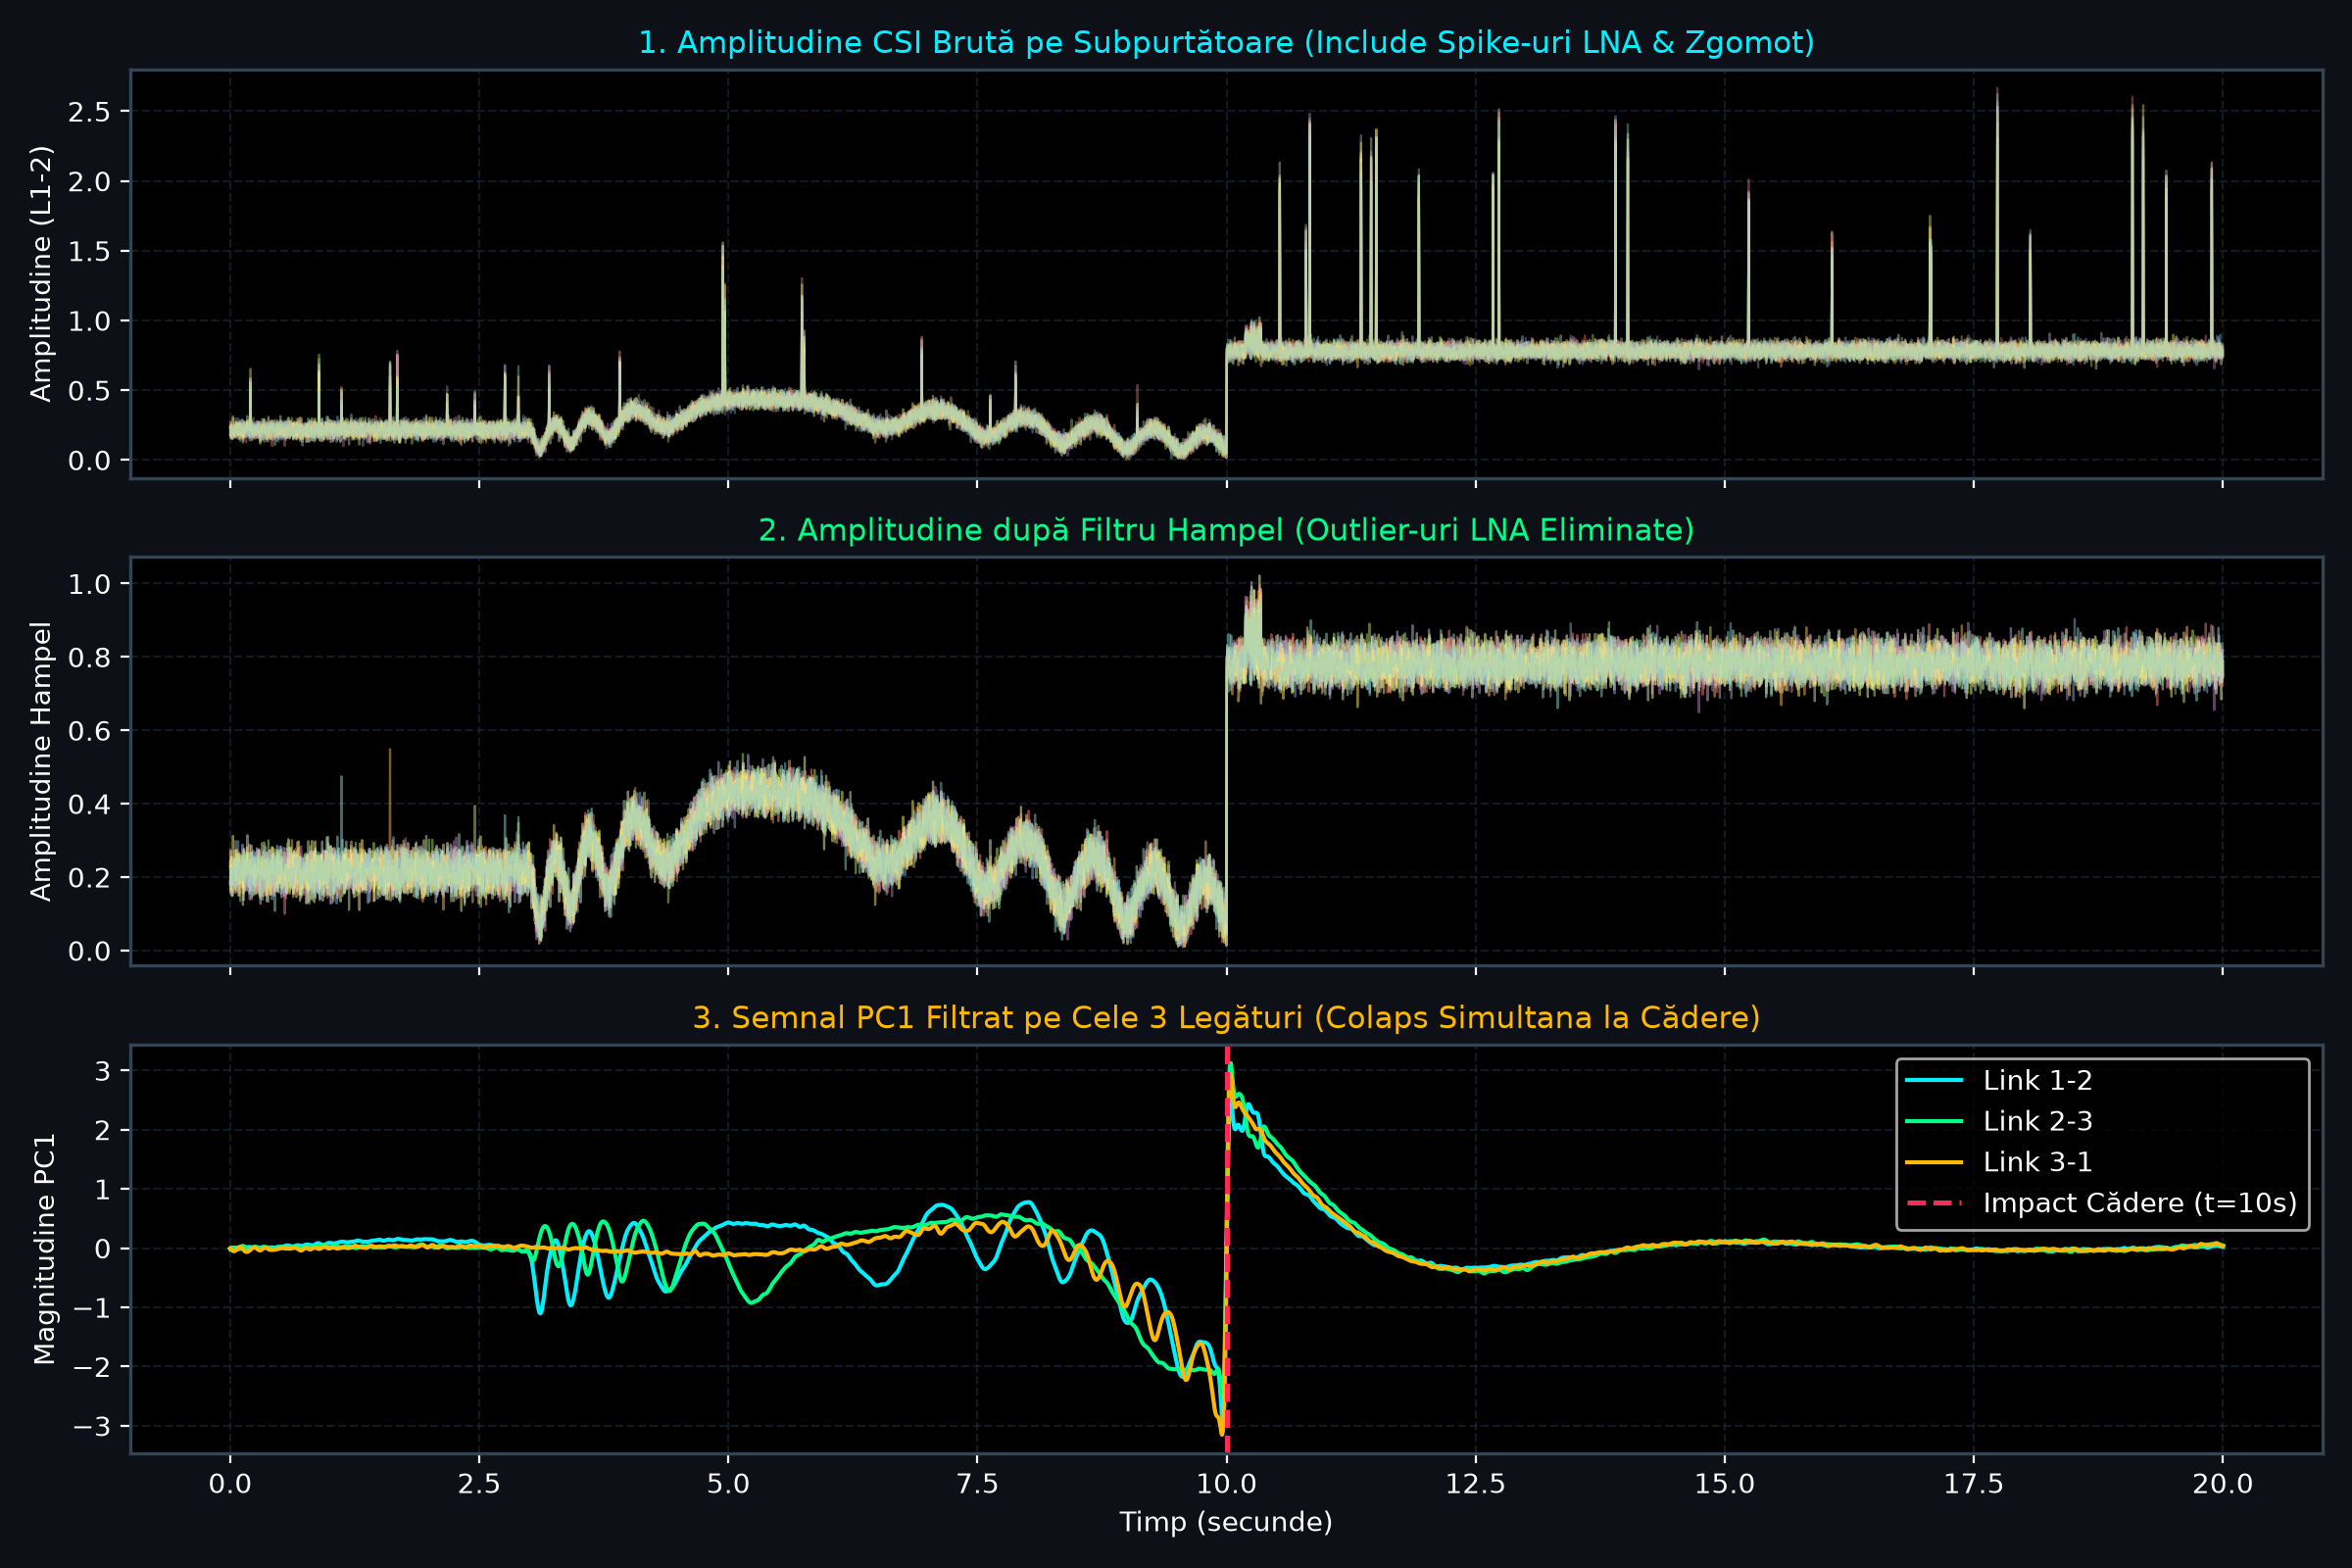
\includegraphics[width=0.95\textwidth]{figures/1_raw_vs_filtered_csi.png}
    \caption{Comparație între semnalul CSI brut și semnalul obținut în urma etapelor de filtrare Hampel, Butterworth și proiecție PCA.}
    \label{fig:raw_vs_filtered}
\end{figure}

\subsection{1. Eliminarea Outlierilor prin Filtrul Hampel}
Filtrul Hampel este un filtru neliniar bazat pe deviația mediană absolută (MAD -- \textit{Median Absolute Deviation}), utilizat pentru eliminarea vârfurilor ascuțite cauzate de comutația AGC a etajului radio fără a distorsiona tranzițiile abrupte de impact.

Pentru un eșantion $x_i$ dintr-o fereastră de lățime $2k+1$ centrată în $i$, se calculează mediana ferestrei $\tilde{x}_i$:
\begin{equation}
    \tilde{x}_i = \text{median}(x_{i-k}, \dots, x_i, \dots, x_{i+k})
\end{equation}
și deviația mediană absolută $S_i$:
\begin{equation}
    S_i = 1.4826 \times \text{median}(|x_{i-k} - \tilde{x}_i|, \dots, |x_{i+k} - \tilde{x}_i|)
\end{equation}
Factorul 1.4826 scalează MAD la valoarea deviației standard a unei distribuții gaussiene. Dacă abaterea eșantionului depășește pragul stabilit:
\begin{equation}
    |x_i - \tilde{x}_i| > 3 S_i
\end{equation}
valoarea $x_i$ este înlocuită cu mediana locală $\tilde{x}_i$. În sistemul nostru s-a utilizat o fereastră de $k = 3$ eșantioane.

\subsection{2. Filtrarea Trece-Bandă Butterworth}
Mișcarea corpului uman induce variații de amplitudine într-o gamă de frecvențe cuprinsă între $0.2\text{ Hz}$ (respirație lentă și pași rari) și $12.0\text{ Hz}$ (brațe și picioare în mișcare rapidă). Variațiile sub $0.2\text{ Hz}$ reflectă deriva termică a componentelor electronice și modificările lente de temperatură ambientală, în timp ce frecvențele peste $12\text{ Hz}$ reprezintă zgomot termic alb.

A fost proiectat un filtru digital Butterworth IIR de ordinul 4 cu răspuns în frecvență maxim neted (fără ondulații în banda de trecere):
\begin{equation}
    |H(j\omega)|^2 = \frac{1}{1 + \left(\frac{\omega^2 - \omega_0^2}{\omega \cdot B}\right)^{2N}}
\end{equation}
unde $N = 4$, $f_{low} = 0.2\text{ Hz}$, $f_{high} = 12.0\text{ Hz}$, iar $B = f_{high} - f_{low}$. Filtrarea a fost aplicată bidirecțional (filtrare cu fază nulă \texttt{filtfilt}) pentru a preveni orice decalaj temporal al momentului de cădere.

\subsection{3. Reducerea Dimensionalității prin Analiza Componentelor Principale (PCA)}
După filtrarea trece-bandă, cele 52 de subpurtătoare conțin informație puternic corelată, dar scalată diferit din cauza fading-ului selectiv în frecvență. Pentru a extrage semnalul comun și a maximiza raportul semnal-zgomot (SNR), se aplică Analiza Componentelor Principale (PCA).

Matricea centrată a amplitudinilor filtrate $X \in \mathbb{R}^{N_s \times 52}$ este proiectată calculând matricea de covarianță $C$:
\begin{equation}
    C = \frac{1}{N_s - 1} X^T X
\end{equation}
Se rezolvă problema vectorilor și valorilor proprii:
\begin{equation}
    C v_j = \lambda_j v_j, \quad j \in \{1, \dots, 52\}
\end{equation}
unde valorile proprii sunt ordonate descrescător $\lambda_1 \ge \lambda_2 \ge \dots \ge \lambda_{52}$.

Prima componentă principală $PC_1$ este dată de proiecția:
\begin{equation}
    PC_1 = X v_1
\end{equation}
$PC_1$ capturează peste $82\%$ din varianța totală indusă de traversarea corpului prin zonele Fresnel, furnizând un semnal scalar robust pentru fiecare legătură radio ($L_{12}, L_{23}, L_{31}$).

\section{Analiza Spectrală Micro-Doppler prin STFT}
Pentru a discrimina între căderea bruscă și activitățile casnice obișnuite, se calculează Transformata Fourier pe Timp Scurt (STFT -- \textit{Short-Time Fourier Transform}) a semnalului mediat pe subpurtătoare $s(t) = \frac{1}{52}\sum_{k=1}^{52} |H_k(t)|$:
\begin{equation}
    \text{STFT}\{s(t)\}(\tau, \omega) = \int_{-\infty}^{\infty} s(t) w(t - \tau) e^{-j \omega t} dt
\end{equation}
unde $w(t)$ este o fereastră Hann de lungime $N_{perseg} = 32$ eșantioane cu suprapunere $50\%$ ($N_{overlap} = 16$).

Densitatea spectrală de putere în decibeli este exprimată prin:
\begin{equation}
    P_{dB}(\tau, f) = 10 \log_{10} \left( |\text{STFT}(\tau, 2\pi f)|^2 + 10^{-12} \right)
\end{equation}
Frecvența Doppler de vârf $f_{D, \max}(\tau)$ este determinată la fiecare pas temporal căutând frecvența peste pragul de zgomot ($10\text{ Hz}$) la care energia atinge un maxim local.

\begin{figure}[H]
    \centering
    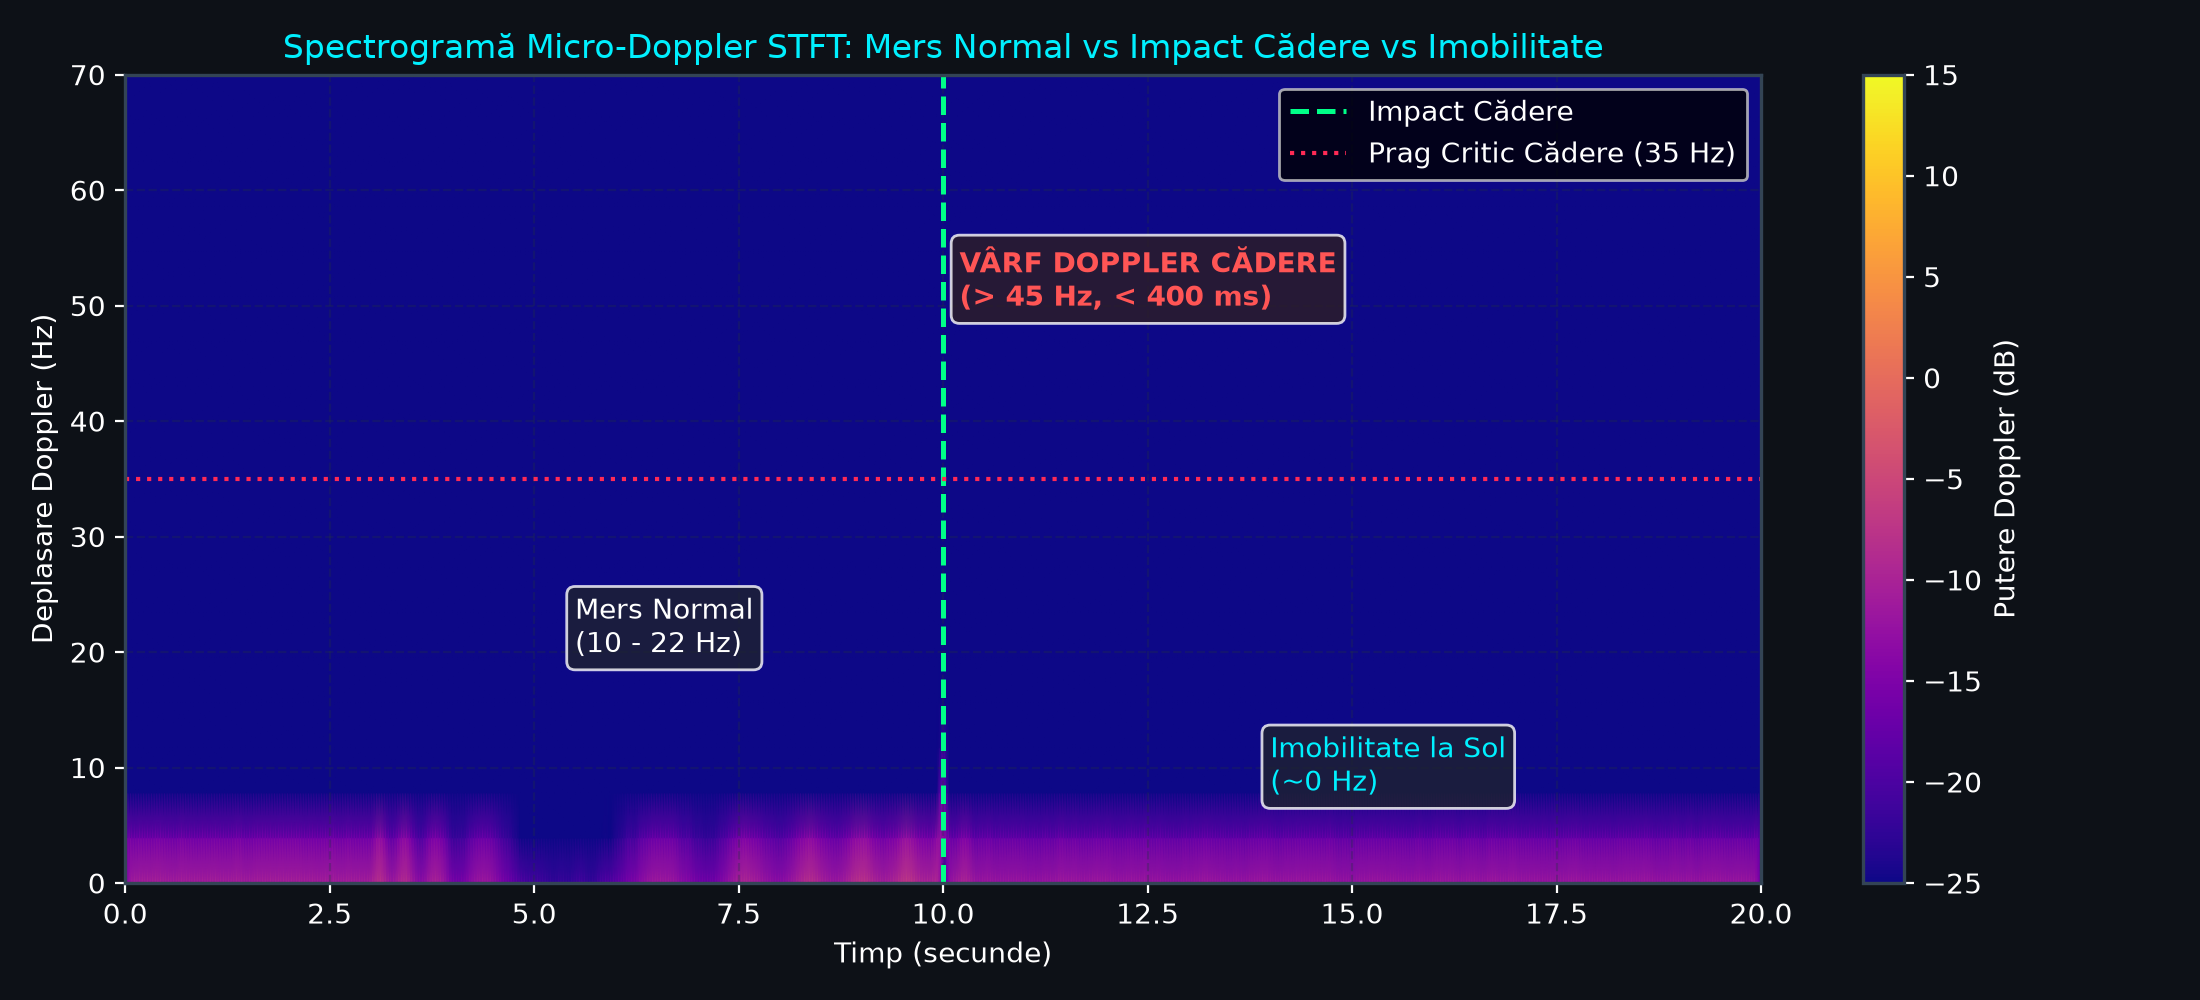
\includegraphics[width=0.95\textwidth]{figures/2_doppler_spectrogram.png}
    \caption{Spectrograma Doppler a căderii: explozia energetică pe frecvențe înalte ($>35\text{ Hz}$) la momentul impactului urmată de platoul de liniște.}
    \label{fig:doppler_spectrogram}
\end{figure}

\section{Automatele cu Stări Finite Analitice (FallDetectorFSM)}
Spre deosebire de modelele de învățare profundă (care necesită mii de eșantioane de antrenare și sunt susceptibile la schimbarea mediului fizic), abordarea noastră folosește un clasificator determinist bazat pe un automat cu stări finite (FSM).

\subsection{Spațiul Stărilor și Condițiile de Tranziție}
Automatul definește 5 stări discrete:
\begin{itemize}
    \item \textbf{Starea 0 (CALM):} Încăpere liniștită, fără mișcare umană semnificativă.
    \item \textbf{Starea 1 (MERS / WALKING):} Deplasare normală a persoanei în încăpere. Modulație energetică cvasi-periodică.
    \item \textbf{Starea 2 (IMPACT DETECTED):} Momentul colapsului fizic. Pante abrupte simultane pe legături și vârf Doppler.
    \item \textbf{Starea 3 (VERIFY DORMANCY):} Fereastră de verificare a imobilității post-impact ($2.5\text{ s}$).
    \item \textbf{Starea 4 (ALARM ACTIVE):} Cădere confirmată definitiv. Persoană la sol fără semne de mișcare voluntară.
\end{itemize}

\begin{figure}[H]
    \centering
    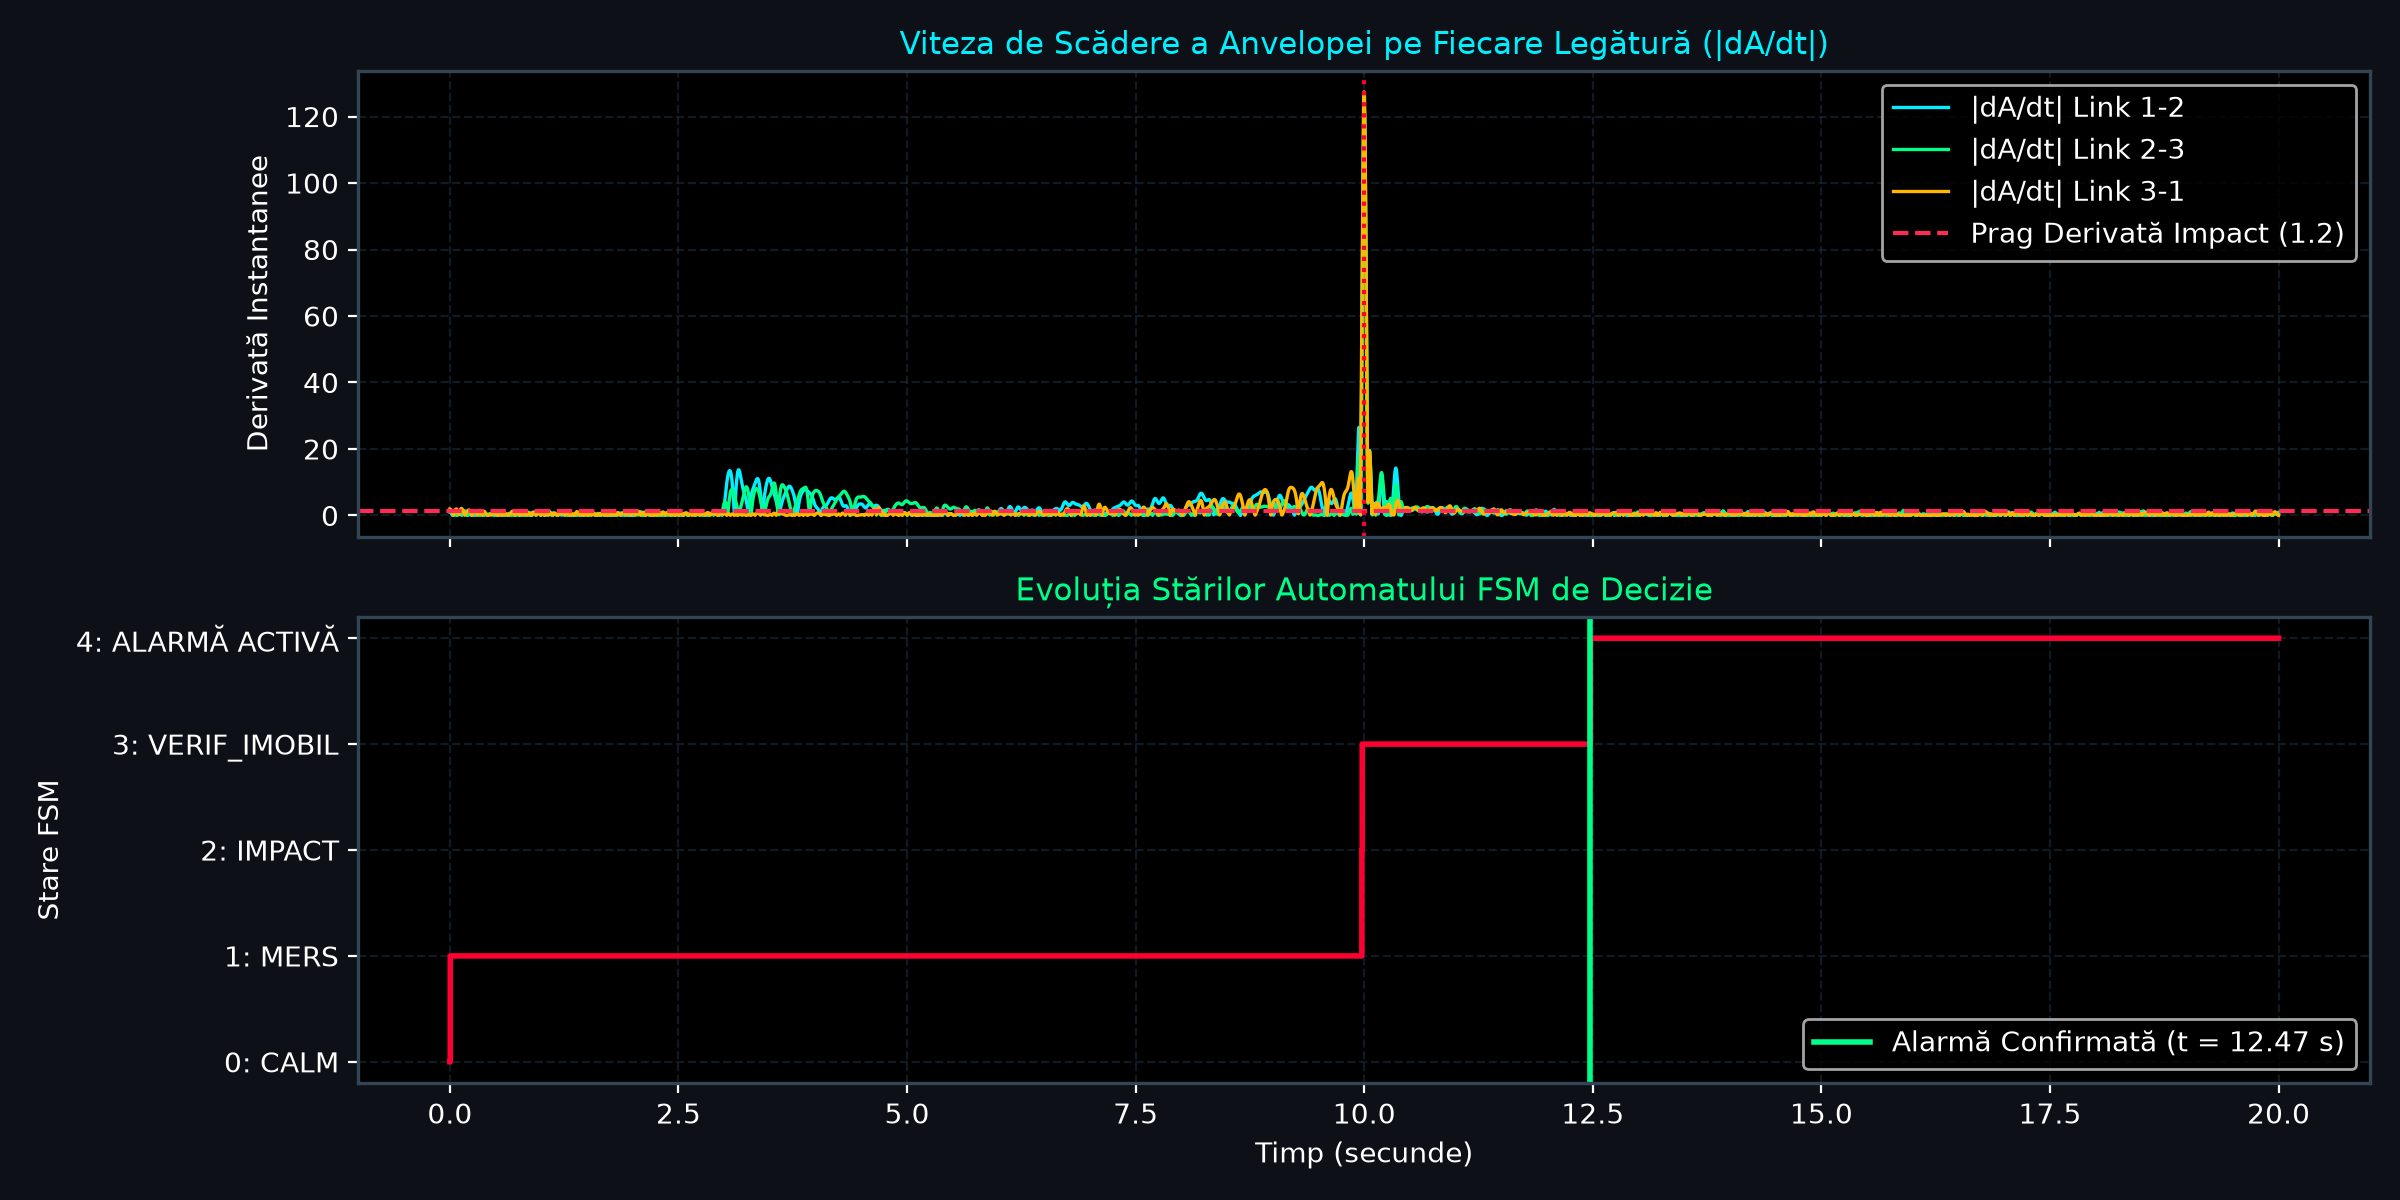
\includegraphics[width=0.95\textwidth]{figures/4_fsm_decision_telemetry.png}
    \caption{Telemetria FSM: tranzițiile dintre stări, derivata $|dA/dt|$ și confirmarea alarmei la finalul ferestrei de imobilitate.}
    \label{fig:fsm_telemetry}
\end{figure}

\subsection{Criteriul de Colaps Simultan Multi-Link}
Pentru fiecare legătură $l \in \{L_{12}, L_{23}, L_{31}\}$, se calculează derivata instantanee a semnalului $PC_1$:
\begin{equation}
    D_l(t) = \left| \frac{d PC_{1, l}(t)}{dt} \right| \approx \left| \frac{PC_{1, l}[i] - PC_{1, l}[i-1]}{\Delta t} \right|
\end{equation}
Semnalele sunt normalizate unitar: $\hat{D}_l(t) = D_l(t) / \max(D_l)$. O tranziție către starea de IMPACT (Starea 2) are loc dacă și numai dacă:
\begin{equation}
    \sum_{l \in \{L_{12}, L_{23}, L_{31}\}} \mathbb{I}(\hat{D}_l(t) > Th_{deriv}) \ge 2 \quad \text{și} \quad \exists l: \hat{D}_l(t) > Th_{violent} \quad \text{și} \quad f_{D, \max}(t) > 35\text{ Hz}
\end{equation}
unde $Th_{deriv} = 0.05$ (normalizat) și $Th_{violent} = 0.15$. Această condiție garantează că un pas izolat (care afectează puternic doar o singură legătură la un moment dat) nu poate declanșa tranziția de impact.

\subsection{Fereastra de Imobilitate Post-Impact (Dormancy Window)}
Odată intrat în Starea 3, algoritmul inițiază un cronometru de $T_{dormancy} = 2.5\text{ secunde}$. În acest interval:
\begin{equation}
    \text{Var}_{post} = \frac{1}{3} \sum_{l} \text{Var}\left(PC_{1, l}[i_{impact} + 0.5 f_s : i_{current}]\right)
\end{equation}
\begin{itemize}
    \item Dacă $\text{Var}_{post} < 0.6$, victima este imobilizată la sol $\rightarrow$ Automatul trece în \textbf{Starea 4 (ALARM ACTIVE)}, emițând alarma de cădere.
    \item Dacă $\text{Var}_{post} \ge 0.6$, utilizatorul s-a ridicat imediat sau continuă mișcarea (de exemplu a scăpat un obiect) $\rightarrow$ Automatul revine în \textbf{Starea 1 (MERS)}, evitând o alarmă falsă.
\end{itemize}
